\documentclass[a4paper,10pt,parskip=half]{scrartcl}
\usepackage[utf8]{inputenc}
\usepackage{listings}
\usepackage{graphicx}
\usepackage{xcolor}

%JSON Listing von http://tex.stackexchange.com/questions/83085/how-to-improve-listings-display-of-json-files
\colorlet{punct}{red!60!black}
\definecolor{background}{RGB}{255,255,255}
\definecolor{delim}{RGB}{20,105,176}
\colorlet{numb}{magenta!60!black}

\lstdefinelanguage{json}{
    basicstyle=\normalfont\ttfamily,
    %numbers=left,
    %numberstyle=\scriptsize,
    stepnumber=1,
    numbersep=8pt,
    showstringspaces=false,
    breaklines=true,
    frame=lines,
    backgroundcolor=\color{background},
    literate=
     *{0}{{{\color{numb}0}}}{1}
      {1}{{{\color{numb}1}}}{1}
      {2}{{{\color{numb}2}}}{1}
      {3}{{{\color{numb}3}}}{1}
      {4}{{{\color{numb}4}}}{1}
      {5}{{{\color{numb}5}}}{1}
      {6}{{{\color{numb}6}}}{1}
      {7}{{{\color{numb}7}}}{1}
      {8}{{{\color{numb}8}}}{1}
      {9}{{{\color{numb}9}}}{1}
      {:}{{{\color{punct}{:}}}}{1}
      {,}{{{\color{punct}{,}}}}{1}
      {\{}{{{\color{delim}{\{}}}}{1}
      {\}}{{{\color{delim}{\}}}}}{1}
      {[}{{{\color{delim}{[}}}}{1}
      {]}{{{\color{delim}{]}}}}{1},
}

%opening
\title{Modellierung Informationssysteme Praktikum}
\subtitle{Schnittstelle zwischen Parser und FB-API Komponente [DRAFT!]}
\author{Lukas Grundmann}
\date{\today}

\begin{document}

\maketitle

\begin{abstract}

\end{abstract}

\section{Änderungen}

\begin{itemize}
 \item \textit{04.11.2014}: Initialer Entwurf von Lukas Grundmann
\end{itemize}

\section{TODO Liste}

Folgend sind noch offene Fragen gelistet:
\begin{itemize}
  \item Selects
  \item Funktionen ausarbeiten
  \item Gewichtungen / Fuzzy Logik durchplanen
\end{itemize}


\section{Einleitung}

Dieses Dokument beschreibt die Schnittstelle zwischen den Komponenten 
\textit{Parser} und {FB-API}. Der \textit{Parser} analysiert die vom Benutzer
gestellte Anfrage und erzeugt dann Ergebnisse im hier festgelegten Format.

\section{Fachlicher Entwurf}

Der Parser erzeugt eine disjunktive Normalform (\textit{DNF}: über 
\textit{oder} verknüpfte boolsche Ausdrücke). Jeder \textit{boolsche Ausdruck} 
der \textit{DNF} besteht aus einem \textit{Attribut} (z.B. Alter eines 
Benutzers), einer (aus Sicht des Parsers) \textit{atomaren Operation} 
(z.B. $<$, $>$, $==$, "in" für Listen, "shows" für Bilderkennung ... siehe 
später) und einem \textit{Wert} in einem bestimmten \textit{Typ} (siehe später).

Folgend eine Liste der aus Sicht des Parsers bekannten \textit{Operationen}:
\begin{itemize}
 \item \textit{$<$, $<=$}: kleiner, kleiner gleich
 \item \textit{$>$, $>=$}: größer, größer gleich
 \item \textit{$==$, $!=$}: gleich, nicht gleich
 \item \textit{in}: sucht ob der Wert des \textit{Attributs} in einer Liste 
    vorkommt
 \item \textit{contains}: prüft ob der folgende Wert sich im Attribut befindet
 \item \textit{shows}: dient zur Bilderkennung
 \item \color{red} ... NOCH WAS VERGESSEN? \color{black}
\end{itemize}

Werte können folgende Typen annehmen:
\begin{itemize}
 \item Primitive: \textit{String}, \textit{Double}
 \item \textit{Listen} über primitive Datentypen (\textit{DoubleList}, 
    \textit{StringList})
 \item Funktion mit Attributliste: Hierüber könnten Ontologien und 
    Schlagworthierarchien wiedergegeben werden \color{red} oder soll das der 
    Parser selber auflösen? \color{black}
\end{itemize}


\textbf{Erweiterung der fachlichen Datenstruktur um Fuzzy Logik:}

Es wird jedem boolschen Ausdruck in Prozent mit übergeben, 
wie stark er bei Berechnung des Werts der gesamten DNF einfließen soll.

\color{red}ZU KLÄREN: Wie sieht die Berechnung der DNF denn dann genau aus?
\color{black}

Abbildung \ref{fig:overview} gibt einen Überblick über die Schnittstelle als 
UML Klassendiagramm.

\begin{figure}[htb]
 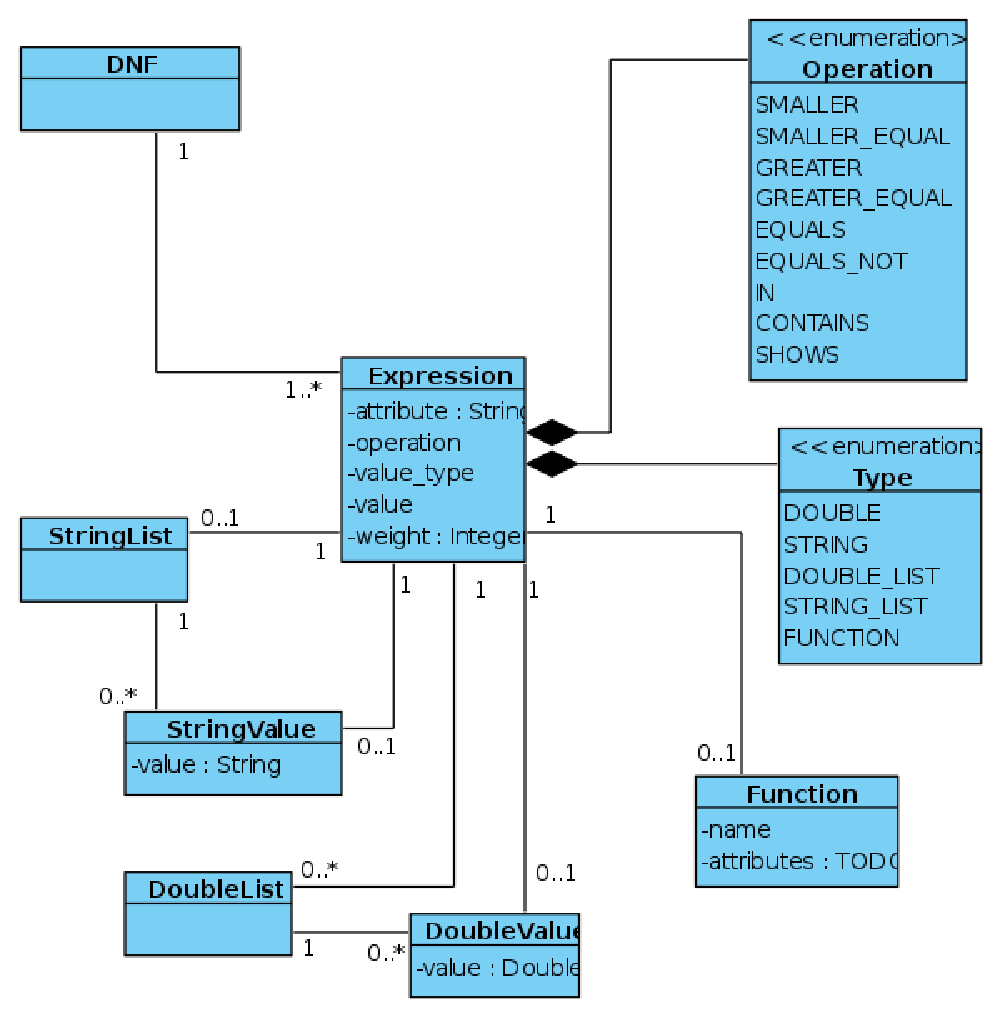
\includegraphics[width=12cm]{overview}
 \caption{UML Überblick über API}
 \label{fig:overview}
\end{figure}


\section{Technischer Entwurf}

Die fachliche Schnittstelle wird über \textit{JSON} abgebildet.

\subsection{JSON Schema}

Es folgt die \color{red}ungetestete \color{black} \textit{JSON} Schema 
Definition:

\begin{lstlisting}[language=json]
{
  "title": "DNF",
  "description": "a disjunctive normal form to select data sets",
  "type": "object",
  "properties": {
    "expressions": {
      "type": "array",
      "minItems": 1,
      "items": {
	"description": "a boolean expression",
	"type": "object",
	"properties": {
	  "weight": {
	    "description": "weight of boolean expression for fuzzy logic",
	    "type":	"integer"
	  },
	  "attribute": {
	    "description": "data attribute involved in boolean expression",
	    "type": "string"
	  },
	  "operation": {
	    "description": "operation used to calculate boolean value",
	    "enum": [ "SMALLER", "SMALLER_EQUALS", "GREATER", 
	      "GREATER_EQUALS", "EQUALS", "EQUALS_NOT", "IN", "CONTAINS",
	      "SHOWS" ]
	  },
	  "value_type": {
	    "description": "type of constant(s) used for operation",
	    "enum": [ "DOUBLE", "STRING", "DOUBLE_LIST", "STRING_LIST", "FUNCTION" ]
	  },
	  "value": {
	    "description": "argument(s) for operation of type value_type",
	    "oneOf": [
	      { "type": "string" },
	      { "type": "double" },
	      {
		"type": "array",
		"items": { "type": "double" },
		"uniqueItems": false"
	      },
	      {
		"type": "array",
		"items": { "type": "string" },
		"uniqueItems": false"
	      },
	      {
		"description": "a function TODO",
		"name": { "type": "string" },
		"arguments": {
		  "type": "array",
		  "uniqueItems": false",
		  "items": {
		    "type": "string"
		  }
		}
	      }
	    ]
	  }
	}
      },
      "uniqueItems": false
    }
  },
  "required": ["weight", "attribute", "operation", "value_type", "value"]
}
\end{lstlisting}

\subsection{Einfaches Beispiel}

\textit{DNF: (user.name in "Nora", "Lukas") || (user.age == 25)}

wird zu folgendem JSON:

\begin{lstlisting}[language=json]
{
    "expressions": [
	{
	    "weight": 100,
	    "attribute": "user.name",
	    "operation": "IN",
	    "value_type": "STRING_LIST",
	    "value": ["Lukas", "Nora"]
	},
	{
	    "weight": 100,
	    "attribute": "user.age",
	    "operation": "EQUALS",
	    "value_type": "DOUBLE",
	    "value": 25
	}
    ]
}
\end{lstlisting}


\end{document}
